\chapter{Software implementado para el sistema}
\label{ape:apendiceC}
En este apartado describiré la aplicación de software utilizada 
para la demostración y validación del este trabajo, la aplicación
fue desarrollada en  el IDE ECLIPSE, como framework para el 
procesamiento de imágenes se utilizó OpenCV, como lenguaje de 
programación nativo se usó c++ y para el diseño de la interfaz de
usuario se utilizó QT. Pasamos a definir los componentes: 

\section{Eclipse IDE}

\begin{wrapfigure}{r}{0.4\textwidth}
  %\begin{center}
    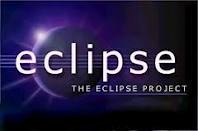
\includegraphics[width=0.4\textwidth]{apendiceC/eclipse}
  %\end{center}
  %\caption{A gull}
\end{wrapfigure}
 
Eclipse es un entorno de desarrollo integrado de código abierto multiplataforma 
para desarrollar lo que el proyecto llama ``Aplicaciones de Cliente Enriquecido", 
opuesto a las aplicaciones ``Cliente-liviano" basadas en navegadores. 
Esta plataforma, típicamente ha sido usada para desarrollar entornos de desarrollo 
integrados (del inglés IDE), como el IDE de Java llamado Java Development Toolkit (JDT) 
y el compilador (ECJ) que se entrega como parte de Eclipse (y que son usados también 
para desarrollar el mismo Eclipse). Sin embargo, también se puede usar para otros 
tipos de aplicaciones cliente, como BitTorrent o Azureus.
Eclipse es también una comunidad de usuarios, extendiendo constantemente las áreas 
de aplicación cubiertas. Un ejemplo es el recientemente creado Eclipse Modeling 
Project, cubriendo casi todas las áreas de Model Driven Engineering.\\
Eclipse fue desarrollado originalmente por IBM como el sucesor de su familia de 
herramientas para VisualAge. Eclipse es ahora desarrollado por la Fundación Eclipse, 
una organización independiente sin ánimo de lucro que fomenta una comunidad de código 
abierto y un conjunto de productos complementarios, capacidades y servicios.
Eclipse fue liberado originalmente bajo la Common Public License, pero después fue 
re-licenciado bajo la Eclipse Public License. La Free Software Foundation ha dicho 
que ambas licencias son licencias de software libre, pero son incompatibles con 
Licencia pública general de GNU (GNU GPL).3 . Para mayor información puede visitar 
el site del proyecto \url{http://www.eclipse.org/}

\section{OpenCV}

\begin{wrapfigure}{l}{0.2\textwidth}
  %\begin{center}
    
\includegraphics[width=0.2\textwidth]{apendiceC/opencv}
  %\end{center}
  %\caption{A gull}
\end{wrapfigure}

OpenCV es una biblioteca libre de visión artificial originalmente desarrollada por Intel. 
Desde que apareció su primera versión alfa en el mes de enero de 1999, se ha utilizado en 
infinidad de aplicaciones. Desde sistemas de seguridad con detección de movimiento, hasta 
aplicativos de control de procesos donde se requiere reconocimiento de objetos. Esto se 
debe a que su publicación se da bajo licencia BSD, que permite que sea usada libremente 
para propósitos comerciales y de investigación con las condiciones en ella expresadas.
Open CV es multiplataforma, existiendo versiones para GNU/Linux, Mac OS X y Windows. 
Contiene más de 500 funciones que abarcan una gran gama de áreas en el proceso de visión, 
como reconocimiento de objetos (reconocimiento facial), calibración de cámaras, visión 
estereo y visión robótica.\\
El proyecto pretende proporcionar un entorno de desarrollo fácil de utilizar y altamente 
eficiente. Esto se ha logrado, realizando su programación en código C y C++ optimizados, 
aprovechando además las capacidades que proveen los procesadores multi núcleo. OpenCV puede 
además utilizar el sistema de primitivas de rendimiento integradas de Intel, un conjunto 
de rutinas de bajo nivel específicas para procesadores Intel.
Para mayor información ver el site \url{http://opencv.willowgarage.com/wiki/}

\section{Qt}

\begin{wrapfigure}{r}{0.3\textwidth}
  %\begin{center}
    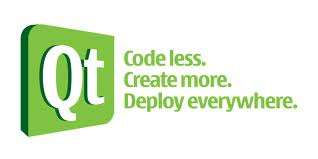
\includegraphics[width=0.3\textwidth]{apendiceC/qt}
  %\end{center}
  %\caption{A gull}
\end{wrapfigure}

Qt es una biblioteca multiplataforma ampliamente usada para desarrollar aplicaciones con 
una interfaz gráfica de usuario así como también para el desarrollo de programas sin 
interfaz gráfica como herramientas para la línea de comandos y consolas para servidores.
Es producido por la división de software Qt de Nokia, que entró en vigor después de la 
adquisición por parte de Nokia de la empresa noruega Trolltech, el productor original 
de Qt, el 17 de junio de 2008.16 Nokia anuncio que va a detener sus desarrollos en Symbian 
para usar la plataforma de Microsoft para sus telefonos inteligentes en Febrero de 2011.
En marzo del mismo año, anunciaron la adquisición de las licencias comerciales de QT por 
Digia PLC, aunque Nokia va a continuar como la fuerza de desarrollo principal atras de 
la librería.\\
Qt es utilizada en KDE, un entorno de escritorio para sistemas como GNU/Linux o FreeBSD, 
entre otros. Qt utiliza el lenguaje de programación C++ de forma nativa, adicionalmente 
puede ser utilizado en varios otros lenguajes de programación a través de bindings. 
También es usada en sistemas informáticos empotrados para automoción, aeronavegación y 
aparatos domésticos como frigoríficos.
Funciona en todas las principales plataformas, y tiene un amplio apoyo. El API de la 
biblioteca cuenta con métodos para acceder a bases de datos mediante SQL, así como uso 
de XML, gestión de hilos, soporte de red, una API multiplataforma unificada para la 
manipulación de archivos y una multitud de otros para el manejo de ficheros, además de 
estructuras de datos tradicionales.
Distribuida bajo los términos de GNU Lesser General Public License (y otras), Qt es 
software libre y de código abierto. Para mayor información visitar el site 
\url{http://qt.nokia.com/products/}

\section{Descripción de la aplicación}
\begin{figure}[h]
 \centering
  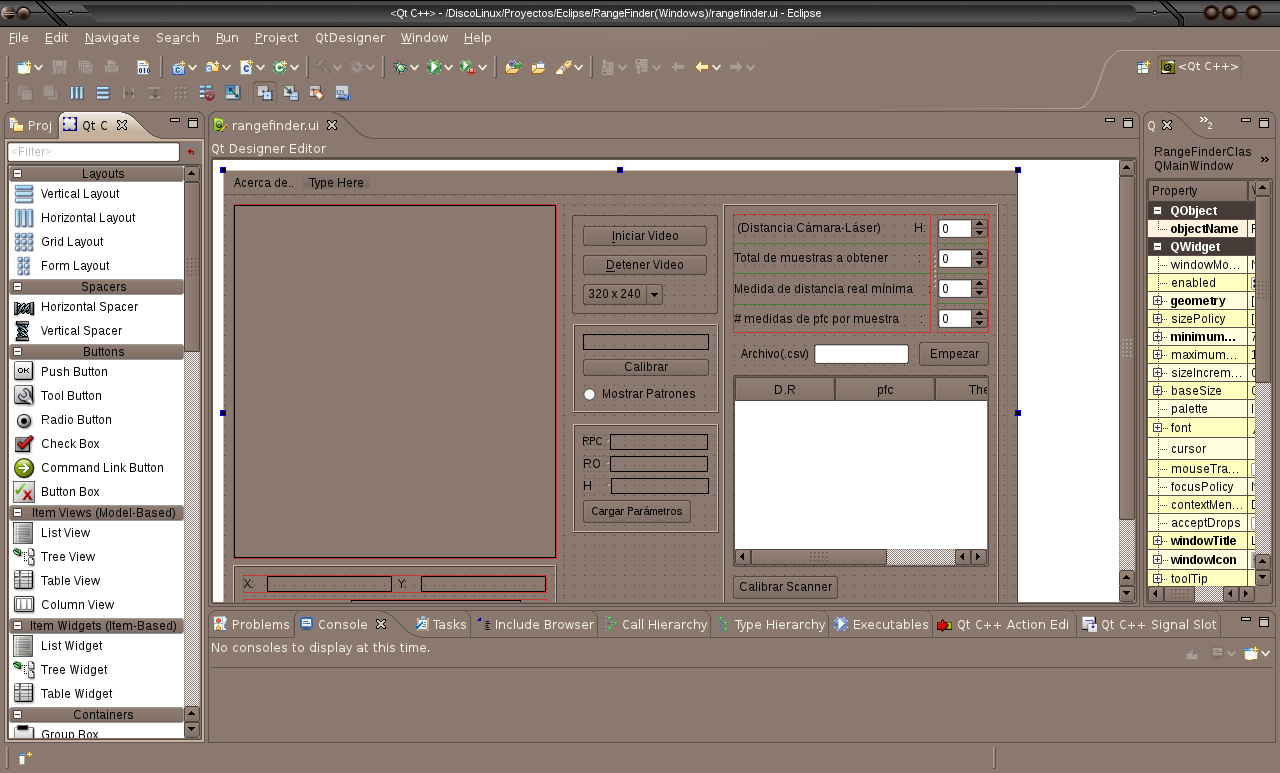
\includegraphics[width=0.7\textwidth]{apendiceC/eclipseintegration}
  \caption{Integración del plugin de Qt para Eclipse, se pueden ver sus cajas de herramientas 
  y su diseñador integrado de interfaces de usuario.}
\label{fig:eclipseintegration}
\end{figure}
El funcionamiento de la aplicación se describe en la Figura \ldots en donde
se puede apreciar el flujo de procesos de la aplicación, el desarrollo de la aplicación se 
hizo en IDE Eclipse Versión Ganymede y la integración de QT con Opencv se llevó a cabo con 
el QT Eclipse Plugin Integration disponible en \url{http://qt.nokia.com/products/eclipse-integration}.
En la Figura \ref{fig:eclipseintegration} podemos ver el plugin de QT integrado en Eclipse, se 
pueden apreciar sus cajas de herramientas y su diseñador integrado de interfaces de usuario.

\subsection{Componentes del sistema}
Para un mejor entendimiento de la estructura de la aplicación se muestra su respectivo Diagrama UML 
de componentes y de clases utilizados en el sistema. 

DIAGRAMA DE COMPONENTES
\begin{figure}[h]
 \centering
  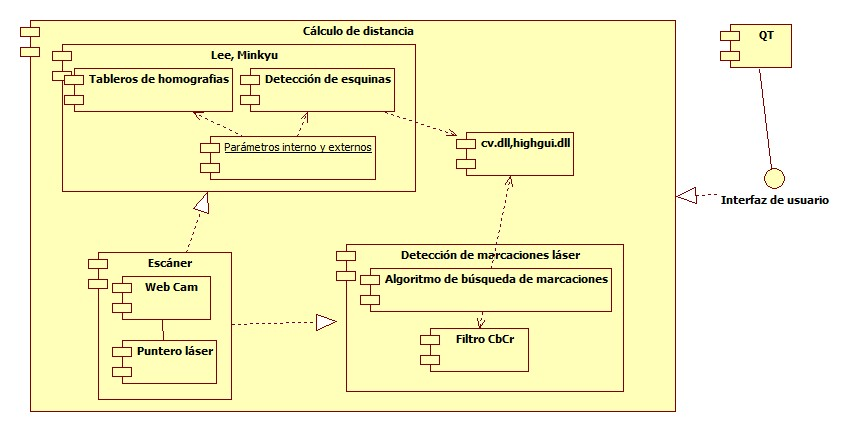
\includegraphics[width=0.9\textwidth]{apendiceC/Componentes}
  \caption{Diagrama de Componentes de la aplicación desarrollado para validación del modelo de estimación de distancia.}
\end{figure}

\begin{sidewaysfigure}
%\begin{figure}[p]
DIAGRAMA DE CLASES
 \centering
  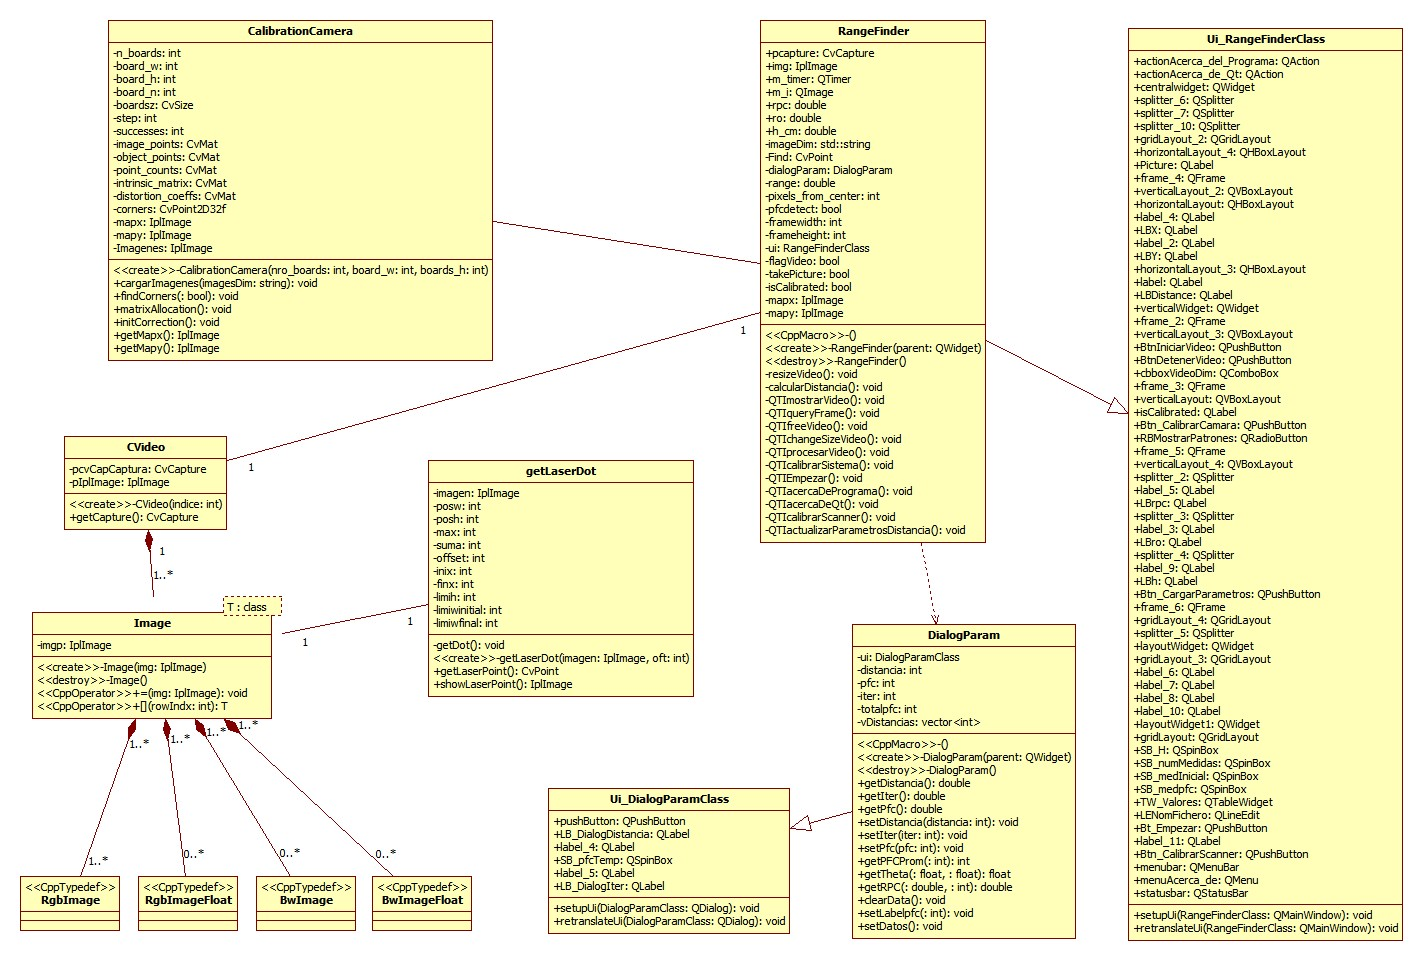
\includegraphics[width=\textwidth]{apendiceC/RangeFinderDiagram}
  \caption{Diagrama de clases de la aplicación desarrollado para validación del modelo de 
estimación de distancia.}
%\end{figure}
\end{sidewaysfigure}




